\section{Controller Design}

%  \begin{table}[H]
%  \begin{tabular}{rl}
%    \texttt{FILES}:         &\texttt{controller.s}  \\
%    \texttt{WRITTEN BY}:    &\texttt{Anand Balakrishnan (anandbal)}
%  \end{tabular}
%  \end{table}


  The \textbf{Controller} mainly contains interrupt handlers, and it is also the entry point for the game.
  In is, we do the following:

  \begin{itemize}
    \item Initialize timer and timer match registers for periodic interrupts.
    \item Listen for UART0 interrupt, read the keystrokes and perform the corresponding action.
    \item Listen for External Interrupt Button press and PAUSE the game.
  \end{itemize}

  The \textbf{Controller} is a relatively small component, responsible mainly for updating the \textbf{Model} via subroutines exposed by the \textbf{Model}. It triggers periodic updates to \textbf{Model} and receives user input, which it queues into \textbf{Model}.
  It's main components are below:

  \begin{figure}[H]
    \centering
    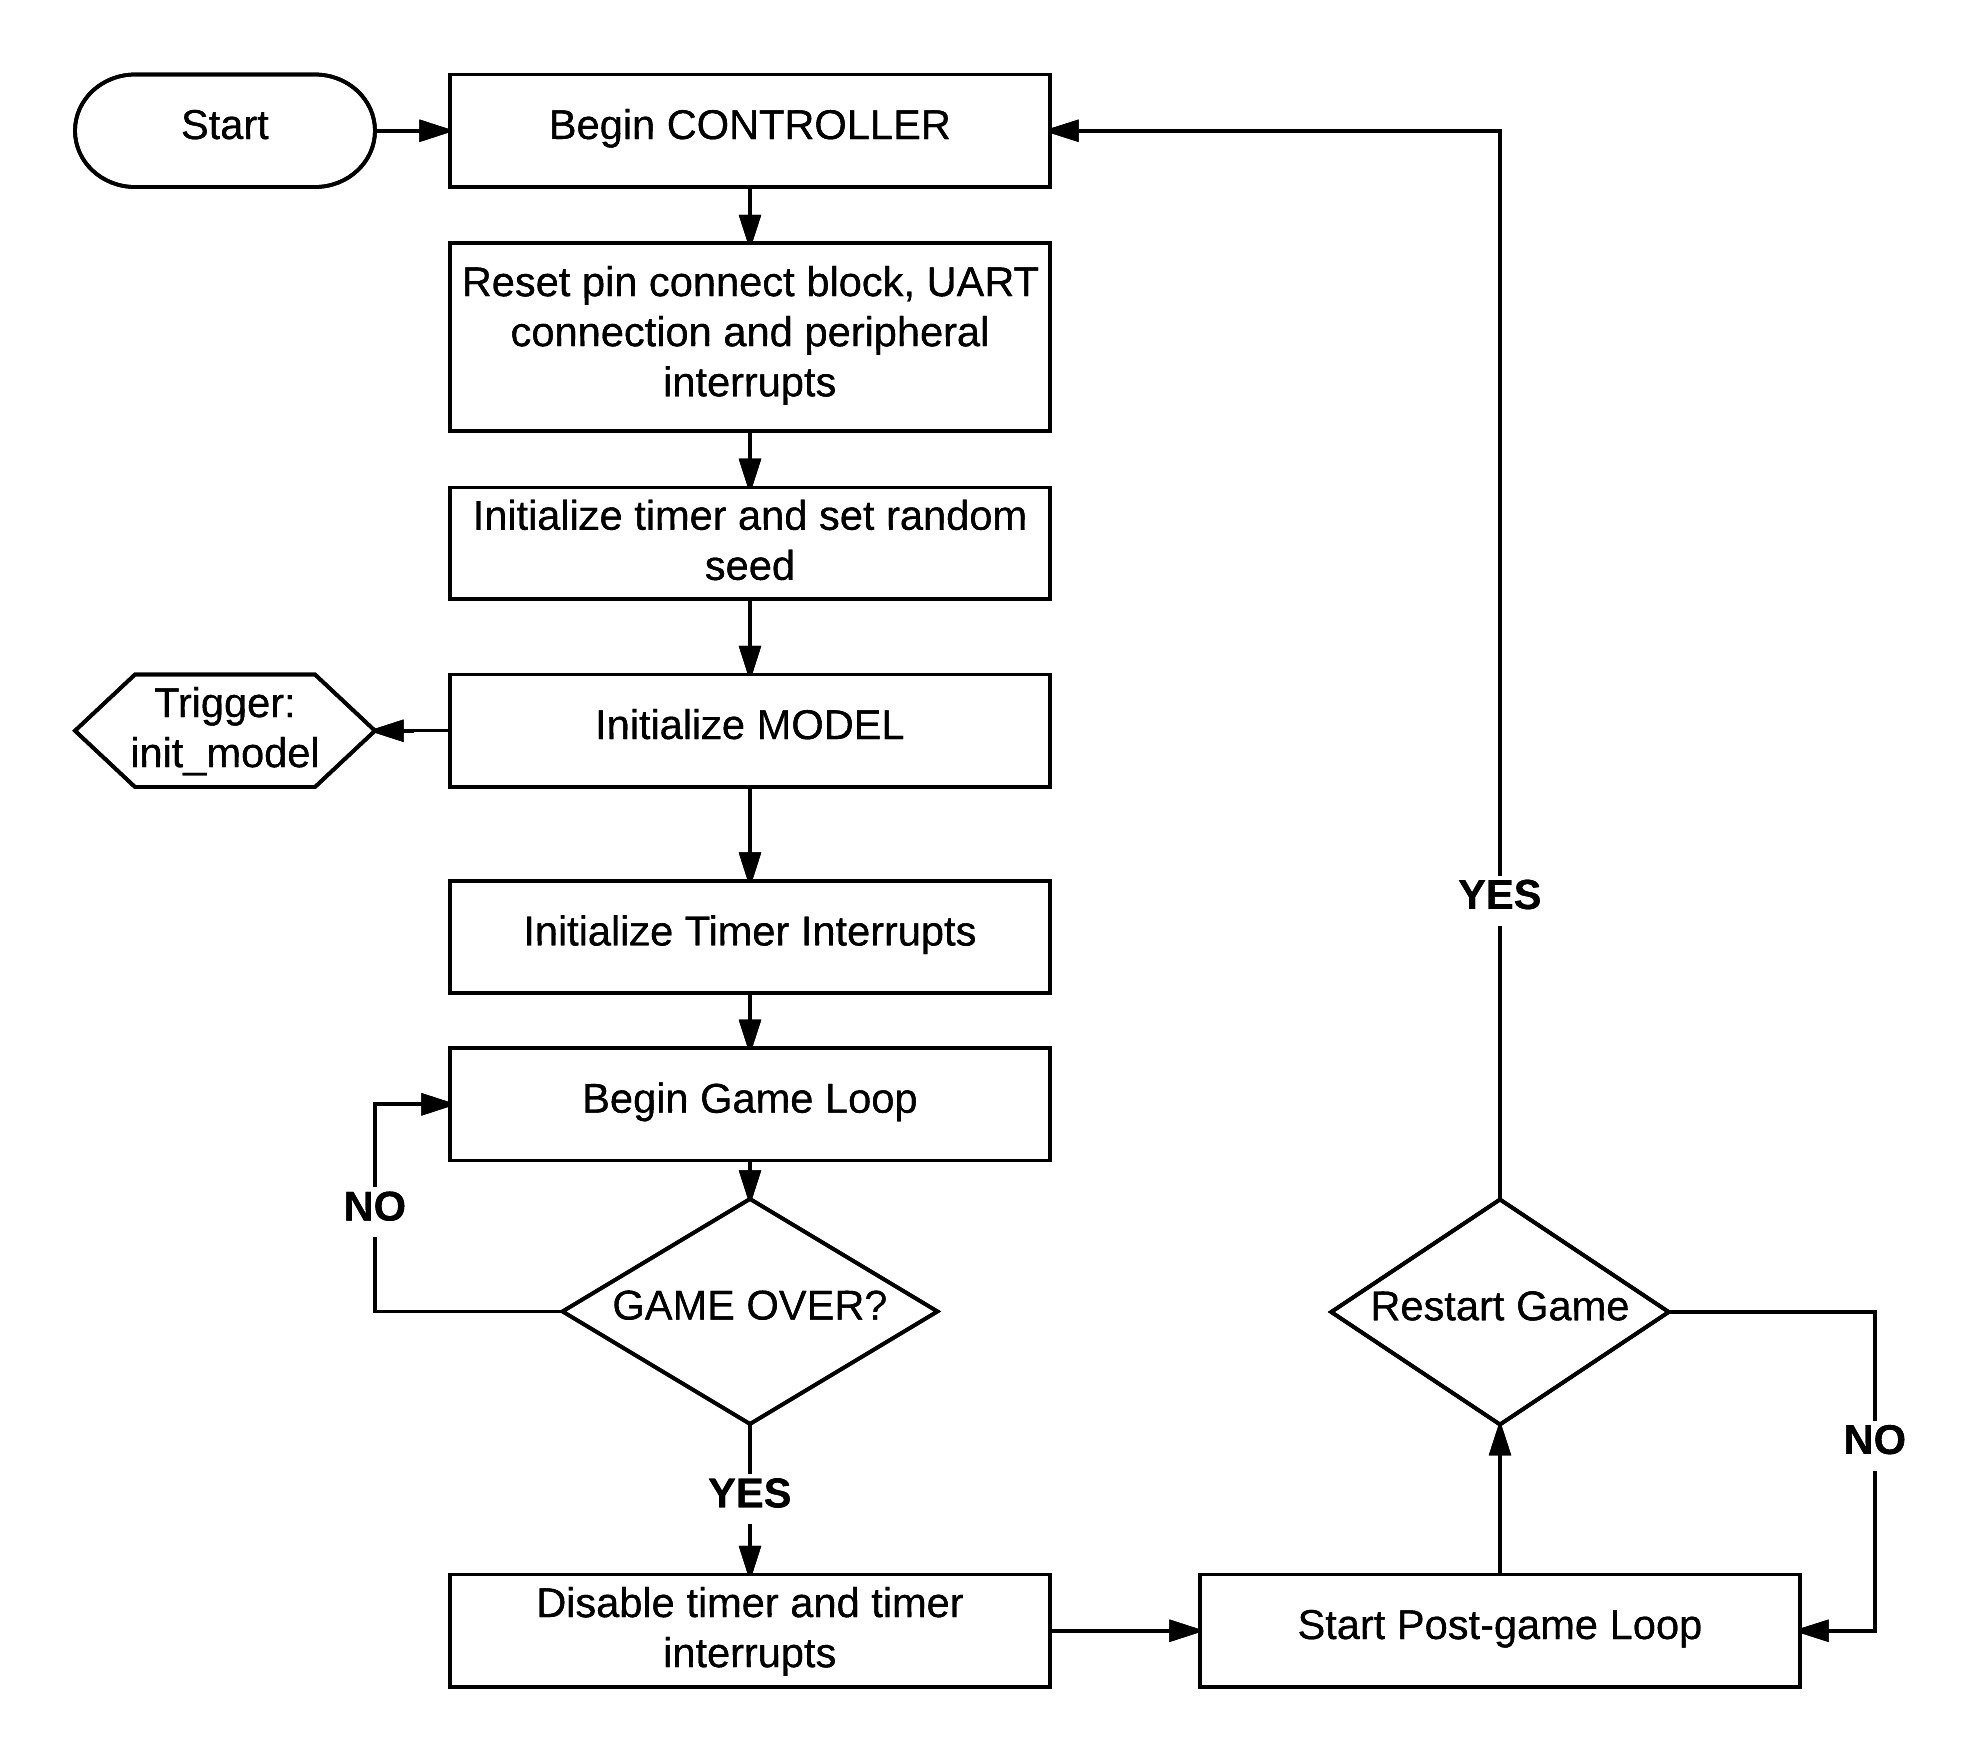
\includegraphics[width=0.9\textwidth]{images/controller-base.png}
    \caption{\label{fig:controller-init} Initialization of \textbf{Controller} and entry point for program}
  \end{figure}

  \begin{figure}[H]
    \centering
    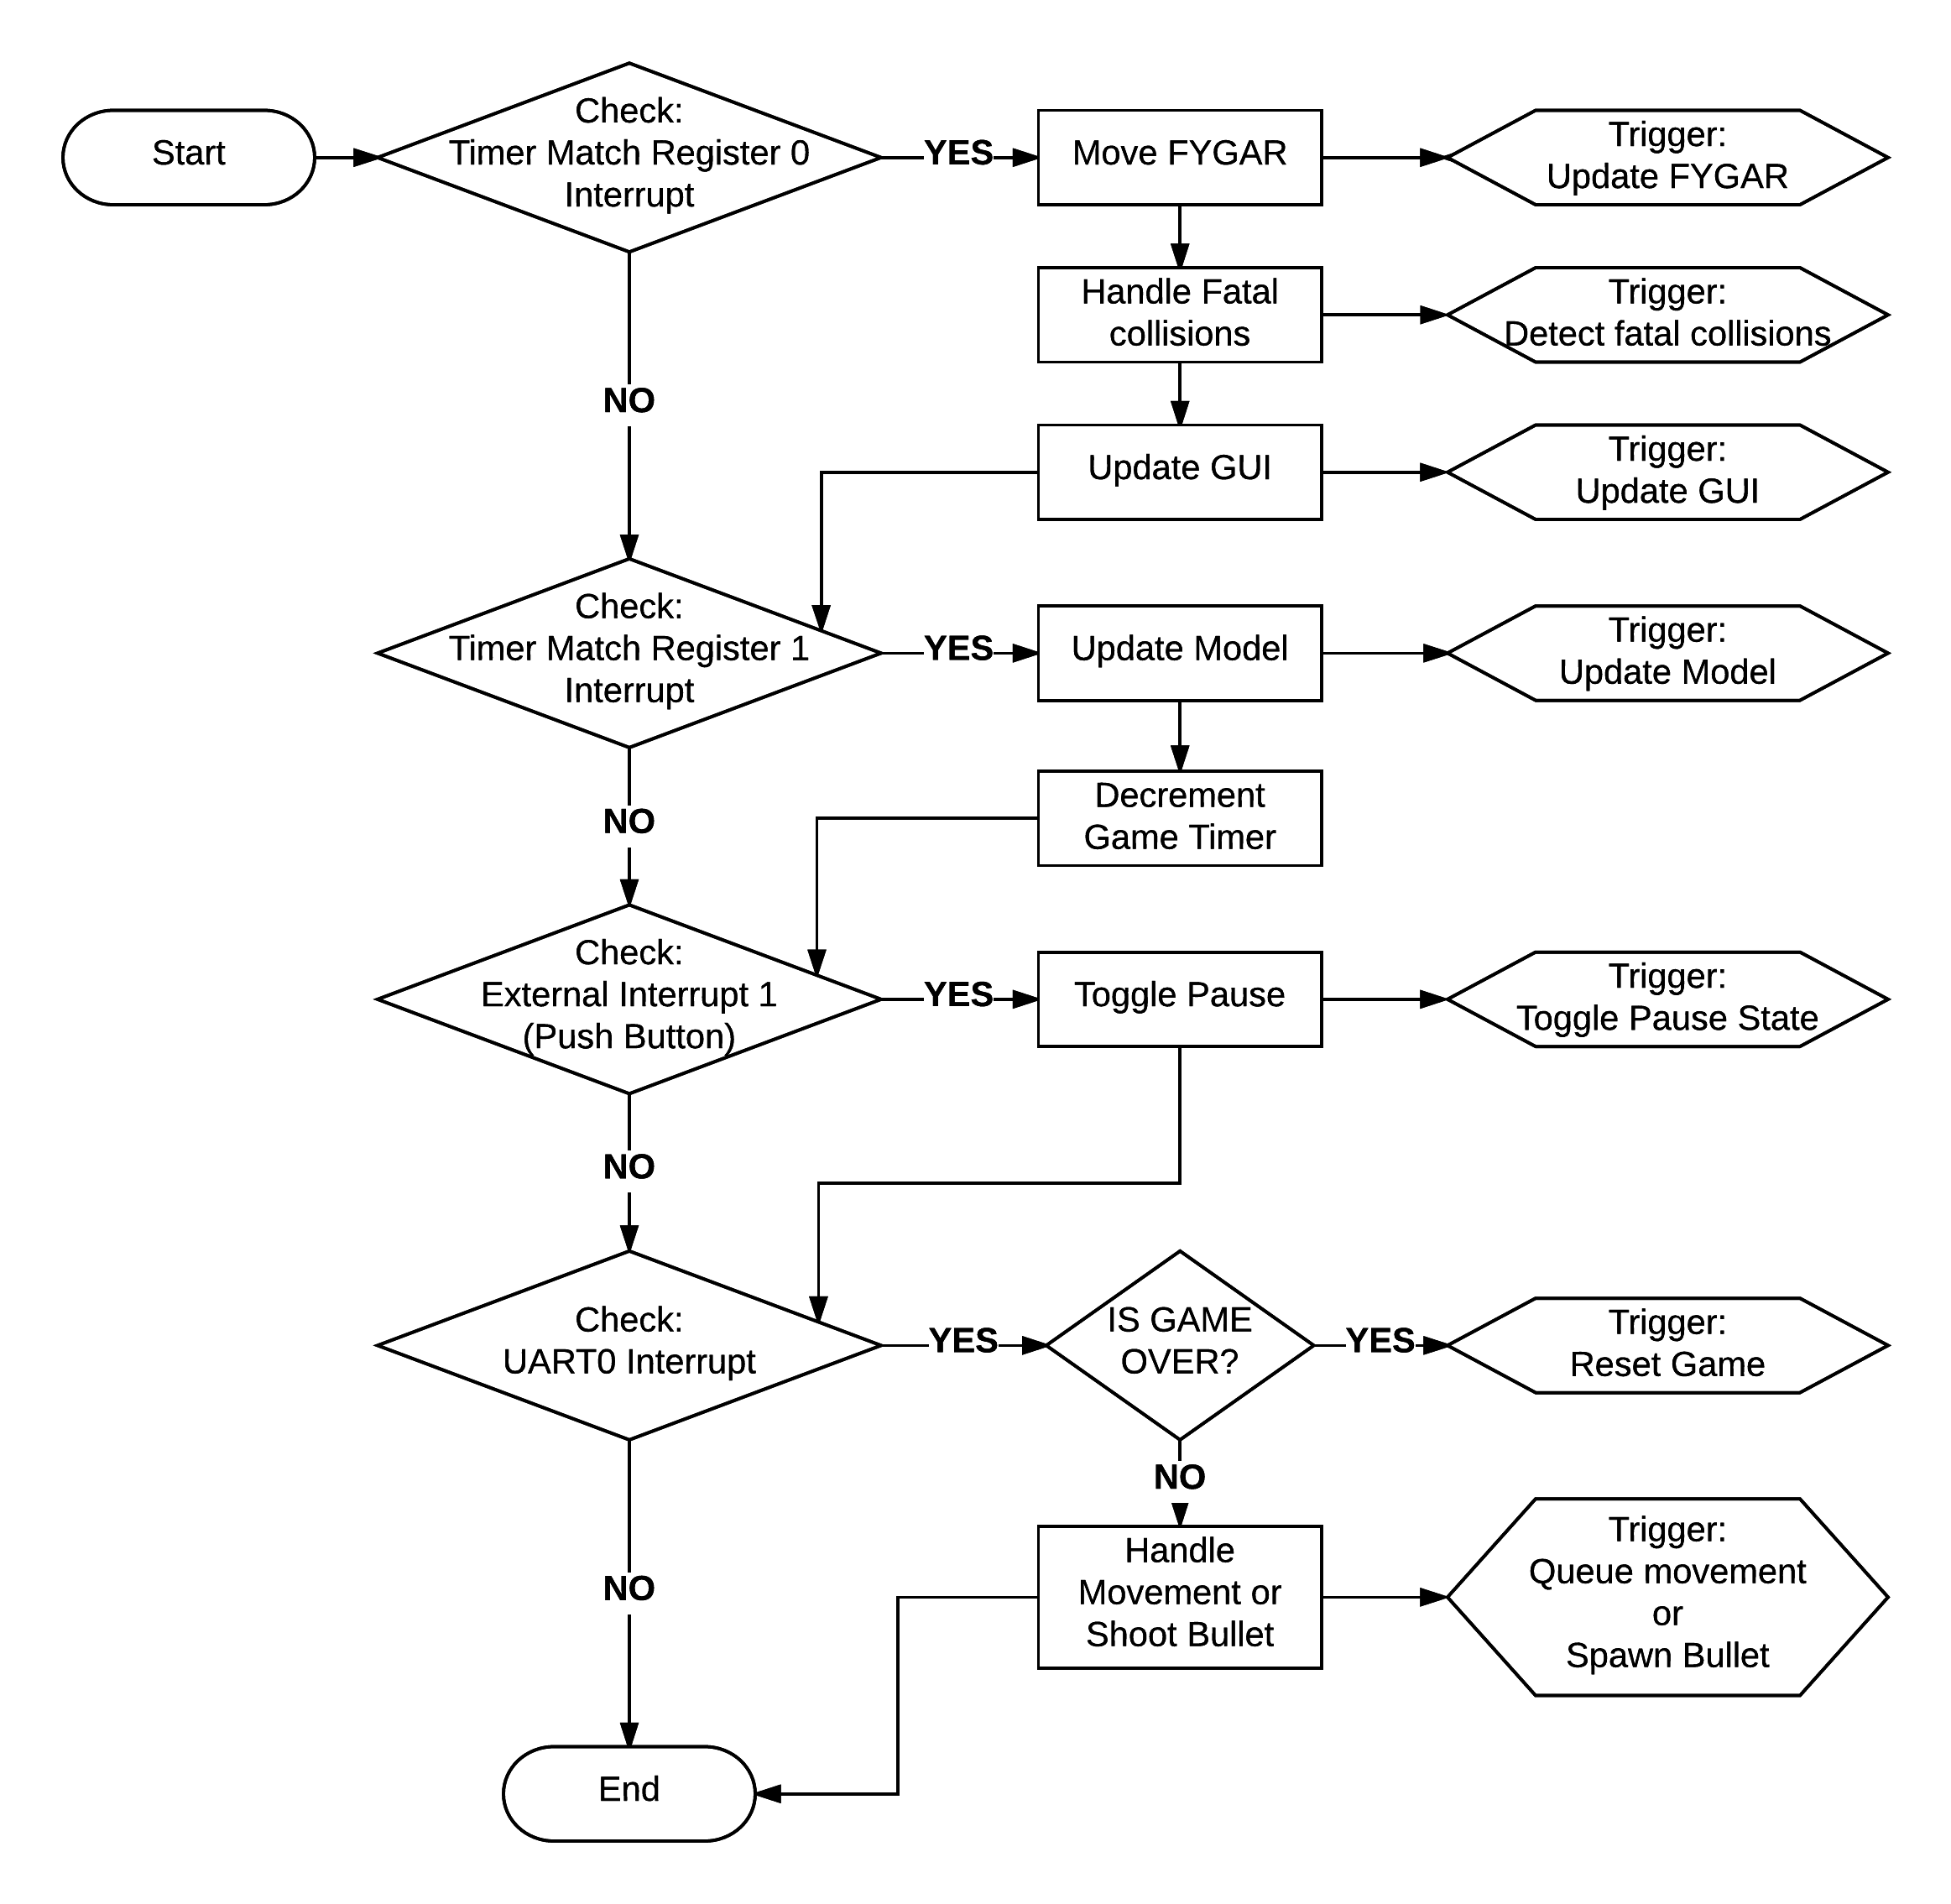
\includegraphics[width=0.9\textwidth]{images/fiq-handler.png}
    \caption{\label{fig:fiq-handler} FIQ Handler to send periodic updates to \textbf{Model} and for listening to user input to control the game.}
  \end{figure}


  While the \textbf{Controller} is only a small part of the application, it is the origin of all triggers. It is the interface between the user and the application.

